\chapter{Erprobung im Labor}\label{cha:Erprobung im Labor}

Nach den anfänglichen Erfahrungen mit Ausfällen von Elektronik und Mechanik bei den ersten Generationen des Flugzeugs, werden alle Komponenten vor dem Einbau einzeln und nach der Montage als System im Labor getestet.
So können der Schadensumfang im Fehlerfall minimiert werden und die Emulation einzelner Betriebsszenarien ermöglicht eine einfache Eingrenzung möglicher Fehlerquellen.
In der Regel werden Szenarien wie die Maximalleistungsaufnahme beim Start und beim  Steigflug sowie das Langzeitverhalten im Reiseflugzustand nachgestellt. Dabei werden relevante Parameter wie Temperatur der Bauteile gemessen und mit den Erwartungen verglichen.

\section{Einzeltests von Baugruppen}

Vor dem Einbau in das Gesamtsystem werden sowohl die einzelnen Platinen als auch ihre Modul Platinen einzeln Ddrchgetestet.
Dazu wird für die Leistungssysteme ein Labornetzteil als Quelle verwendet welches 0 - 45 V und 0 - 50 A zur Verfügung stellen kann.
Der theoretische Nutzbereich des 4-zelligen Akkusystems von 4,20 V bis 3,00 V je Zelle \footnote{\cite[Seite~1.12f.]{Reddy2010}} stellt einen Operationsbreich von 16,8 V bis 12,0 V bereit. Deshalb wird für die meisten Tests eine mittlere Spannung von 14,5 V gewählt. Der Strom wird auf etwa 30 A begrenzt um mögliche Fehlerfolgen zu begrenzen.
Die als kritisch eingestuften Bauteile werden mit Thermoelementen vom Typ K beklebt. Außerdem wird eine FLIR Thermokamera mit einer Auflösung von 320x240 Pixel fest aufgestellt, um die globale Themperaturverteilung auf dem PCB zu beobachten.
Da die absolute Genauigkeit der Temperaturwerte der Wärmebildaufnahmen aufgrund des ungekühlten CCD zumeist nicht korrekt sind, werden diese mit Hilfe der genauen Werte der K Elemente skaliert.
Die Temperatur ist in unserem Leistungsbereich die primäre Schadensursache. 
Um eine vergleichbare Kühlungssituation aller getesteten Bauteile zu realisieren, werden diese in der Ebene in ruhiger Luft vermessen und auf Referenz-Grundplatinen montiert.
Dies ermöglicht eine konservative Einordnung des Betriebspunktes, da im Flugbetrieb alle Elektronikkomponenten vom Fahrtwind überspült werden und damit von einer verbesserten Kühlung auzugehen ist.

\subsection{Ideale Diode}

Die Messungen an dem Aufbau des Moduls der Idealen Diode beschränken sich auf das Verhalten als Leistungsbauteil. 
In Anlehnung an die Referenz-Testaufbauten welche von Texas Instruments, Vishay Semiconductors und Toshiba Power Electronics für einzelne Mosfets in den zugehörigen Datenblättern verwendet werden, ist auch die Adapterplatine für alle Idealen Dioden gestaltet.
Die Platine misst 1x1 Zoll mit 35 um Kupferstärke und regulärem Lötstopplack. Die Ein- und Ausgänge sind über Powerpol 55A Steckverbinder realisiert. SMD montierte Ösen ermöglichen den Abgriff der Differenzspannung über das gesamte Ideale Dioden Modul. In Einzelfällen wird zum Vergleich der Spannungsabfall über den reinen Mosfet manuell zum Vergleich gemessen.

Die vergleichende Messung der beiden Generationen und verschiedener Mosfet-Bestückungen zeigt die unterschiedlichen equivalenten Widerstände über den durchgeleiteten Strom.
Dieser Strom ist unmittelbar nach den Ohmschen Gesetzen für die örtliche Verlustleistung und damit für die Erwärmung der Baugruppe verantwortlich.

\begin{figure}[H]
\centering
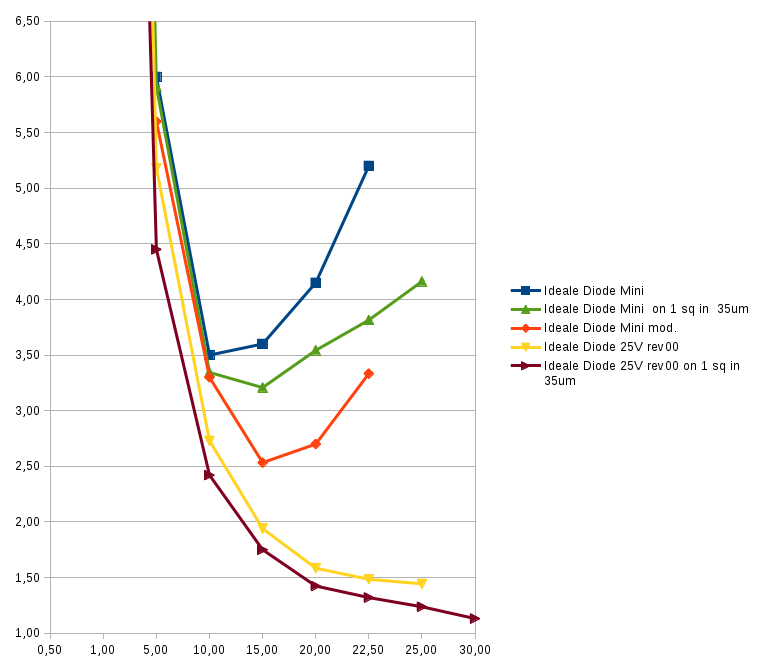
\includegraphics[width=0.9\textwidth]{graphen/Wiederstand-Strom-Ideale_Diode_ver00} 
\caption{Widerstandsverlauf} 
\label{fig:Widerstandsverlauf}
\end{figure}


Wie aus der Grafik \ref{fig:Widerstandsverlauf} ersichtlich wird, ist der Mosfet, wie erwartet, als zentrales Schaltelement für quasi den gesamten Widerstand verantwortlich.
Eine Modifikation der ersten Diodengeneration mit dem Austausch des Mosfet TPN2R304PL mit einem Nennwiderstand von 1,8\,$m\Omega$ \cite{TPN2R304PL} durch den Mosfet FDMC012N03 mit einem Nennwiderstand von 1,36\,m$\Omega$ \cite{FDMC012N03} reduziert den equivalenten Widerstand bei einem üblichen Akkustrom von 10 A im Dauerbetrieb von 3,5\,$m\Omega$  auf 3,2\,$m\Omega$.
Demgegenüber stellt die zweite Generation eine deutliche Widerstandsersparnis dar.
Erreicht wird diese durch ihre optimierte Wärmeableitung mit Neuanordnung der Bauteile und Verkleinerung des PCB sowie der nochmals veränderten Wahl des Mosfets auf TPHR6503PL.

Der höchste Dauerstrom liegt bei der unmodifizierten Generation 1 bei 20\,A und bei der Generation 2 bei 30\,A. 
Generell wird der höchste Dauerstrom über die Baugruppe durch einen kleinstmöglichen Innenwiderstand des verwendeten Mosfets und die Kupferfläche begrenzt, auf welcher das Modul montiert is,t um Wärme abstrahlen zu können. Das Modul PCB selbst hat aufgrund seiner geringen Größe eine vernachlässigbar kleine Kühlleistung.

Das Bild \ref{fig:Beide Generationen des Ideale Dioden Moduls nebeneinander} zeigt zum Vergleich auch das Modul ohne Adapterplatine.

\subsection{5 Volt Servoversorgung}

Um die Eignung der zugekauften 5 V Spannungswandler zu evaluieren, wurde exemplarisch ein Wandler mit einem Servo impulsmäßig belastet.
Dabei wurde das Dc-Dc Modul mit 14,5 V versorgt und an den auf 5,0 V eingestellten Ausgang ein Servo angeschlossen. Der Servo wurde von einem Servo Testgerät mit Steuersignalen versorgt, welche ihn im Wechsel zu den jeweiligen Extrempositionen seines Verfahrbereichs dirigieren. 
An den 5,0 V Ausgang des Wandlers und das in den Servo laufende PWM Signal wurde ein  Digitaloszilloskop angeschlossen. Damit  wurde der Einbruch der 5 V Spannung, unter der impulsartigen Strombelastung, des im Umkehrpunkt beschleunigenden Servos beobachtet.
Damit sollte beurteilt werden, ob der durch die Regelgeschwindigkeit und die begrenzte Ausgangskapazität des Wandlers unvermeidbare kurzzeitige Einbruch im Millisekundenbereich in der Spannungsversorgung der Servos kritische Zustände verursacht.
Es könnte beispielsweise ein zeitgleiches Ausschlagen mehrerer Servomotoren dazu führen. dass die Spannung so weit absinkt, dass keiner der Motoren noch funktionsfähig ist, beziehungsweise die Verfahrgeschwindigkeit deutlich absinkt.

Die Messung ergab einen kumulierten Einbruch der Spannung  unter ca. 0,5 V. 
Damit kann das Verhalten in allen erwarteten Flugsituationen als unkritisch bewertet werden. Gegebenenfalls wird hier in Zukunft zur weiteren Absicherung des Verhaltens noch eine Stützung mit Elektrolythkondensatoren umgesetzt. 

\section{Evaluierung der Signalpfade}

Es sollten Fehler im Schaltplan und im Routing der Platine ausgeschlossen werden. Dafür erfolgte ein Test der korrekten Signalführung ohne Einsatz der Sensoren und der Pixhawk Autopiloten Hardware. Dazu wurden an die Aus- und Eingänge des Pixhawk und der Sensoren ein 1 khz 50 Prozent PWM Signal angelegt, um mit dem Oszilloskop die jeweils vorgesehene Gegenstelle zu überprüfen.

Dabei konnten auf der Autopiloten-Platine keine Fehler festgestellt werden.
Auch die Inbetriebnahme der Sensoren und des Autopiloten verlief Hardwareseitig problemlos.

\section{Überprüfung der Logikfunktionen der Leistungsplatine}

Um eine einwandfreie Funktion und damit den sicheren Betrieb der Leistungsplatine sicherzustellen wurden deren Schutz und Regelfunktionen einzeln getestet.
Es wurden zunächst von einem Paket, aufsteigend, alle Permutationen an Spannungsquellen an die drei vorgesehenen Anschlüsse gekoppelt und die korrekte Führung der Energie überprüft.
Es wurde die vorgesehene Statusindikation durch Leuchtdioden verschiedener Farben dokumentiert.
Die reguläre Führung der Quellen, Blockierung der Flugakkus im Bodenbetrieb und die Anzeige der Energiepfade funktionierte korrekt.

\section{Testlauf der Leistungsplatine}

Anschließend wurde die Platine in den Eingangs beschriebenen Flugmodi im Dauerlauf getestet.
Bei den Tests im Startleistungsbereich stieg der Strom dabei auf einen Wert an, der dazu führte, dass der Sicherungsschalter in Richtung Motorversorgung abschaltete.
Dies führte zu einer Oszillation des zugehörigen Mosfets zwischen Sperr- und Leitzustand. Der in diesem Übergangsbereich hohe Innenwiderstand und der damit verbundene hohe Leistungsabfall am Mosfet führte bereits nach kurzer Zeit zur dessen Zerstörung durch Überhitzung.
Alle weiteren Versuche, dieses Verhalten durch Dämpfung der Abschaltzeitschwelle oder Verbesserung der Kühlung zu vermeiden, blieben erfolglos. Deshalb wurden aufgrund der geringen verbleibenden Zeit bis zum Wettbewerb diese Schaltung ersatzlos entfernt und mit einer entsprechenden Drahtbrücke überbrückt.